%%%%%%%%%%%%%%%%%%%%%%%%%%%%%%%%%%%%%%%%%%%%%%%%%%%%%%%%
% Este é um documento que servirá de modelo para
% os relatórios feitos na disciplina Laboratório de Circuitos Lógicos
% 2020-2
%%%%%%%%%%%%%%%%%%%%%%%%%%%%%%%%%%%%%%%%%%%%%%%%%%%%%%%%%

%%%%%%%%%%%%%%%%%%%%%%%%%%%%%%%%%%%%%%%%%%%%%%%%%%%%%%%%%
% Use os diferentes diretórios para colocar os relatórios de cada experimento, deste modo vc consegue manter um histórico e todo material organizado em apenas um local.
% Lembre-se de mudar o Main Document no Menu!!!

\documentclass[12pt]{article}

\usepackage{sbc-template}
\usepackage[brazil,american]{babel}
\usepackage[utf8]{inputenc}

\usepackage{graphicx}
\usepackage{url}
\usepackage{float}
\usepackage{listings}
\usepackage{color}
\usepackage{todonotes}
\usepackage{algorithmic}
\usepackage{algorithm}
\usepackage{hyperref}
\usepackage{amsmath}
\usepackage{graphicx}
\usepackage{array}
\usepackage{mwe}
\usepackage[shortlabels]{enumitem}

\usepackage{xcolor}
\usepackage{listings}
\usepackage[electronic]{ifsym}
\definecolor{vgreen}{RGB}{104,180,104}
\definecolor{vblue}{RGB}{49,49,255}
\definecolor{vorange}{RGB}{255,143,102}

\lstdefinestyle{verilog-style}
{
    language=Verilog,
    basicstyle=\small\ttfamily,
    keywordstyle=\color{vblue},
    identifierstyle=\color{black},
    commentstyle=\color{vgreen},
    numbers=left,
    numberstyle=\tiny\color{black},
    numbersep=10pt,
    tabsize=8,
    moredelim=*[s][\colorIndex]{[}{]},
    literate=*{:}{:}1
}

\makeatletter
\newcommand*\@lbracket{[}
\newcommand*\@rbracket{]}
\newcommand*\@colon{:}
\newcommand*\colorIndex{%
    \edef\@temp{\the\lst@token}%
    \ifx\@temp\@lbracket \color{black}%
    \else\ifx\@temp\@rbracket \color{black}%
    \else\ifx\@temp\@colon \color{black}%
    \else \color{vorange}%
    \fi\fi\fi
}
\makeatother

\usepackage{trace}

\sloppy


\title{Projeto Final\\
ZeptoProcessador-III de 16 Bits}

\author{Matheus Cardoso de Souza, 202033507\\
        Ualiton Ventura da Silva, 202033580\\
        Grupo G42
}

%%%% LEMBRE-SE DE MUDAR O GRUPO NA LINHA ABAIXO!!!!! %%%%%%
\address{Dep. Ciência da Computação -- Universidade de Brasília (UnB)\\
  CIC0231 - Laboratório de Circuitos Lógicos
  \email{matheus-cardoso.mc@aluno.unb.br, 202033580@aluno.unb.br}
}

\begin{document}
\maketitle

\selectlanguage{american}
 \begin{abstract}
   \textbf{TODO}
 \end{abstract}

\selectlanguage{brazil}
 \begin{resumo}
   O presente relatório apresentará uma descrição detalhada de todos os
   processos que abrangem a construção de um processador, um dos circuitos
   lógicos mais importantes na atualidade.

   \textbf{TODO}
 \end{resumo}


\section{Introdução}\label{sec:Introducao}

\textbf{TODO}

\subsection{Objetivos}\label{sec:Objetivos}

\textbf{TODO}

\subsection{Materiais}\label{sec:Materiais}

Em função da natureza do ensino a distância, os presentes experimentos não foram
realizados usando-se materiais e equipamentos físicos, mas sim emulados por meio
do software
\href{https://www.digitalelectronicsdeeds.com/downloads.html}{Deeds}.

A seguir estão enumerados os materiais utilizados:
\begin{itemize}
    \item Software Deeds
    \item Portas lógicas
    \begin{itemize}
      \item Portas Lógicas \emph{AND}
      \item Portas Lógicas \emph{NAND}
      \item Portas Lógicas \emph{NOR}
      \item Portas Lógicas \emph{OR}
    \end{itemize}
    \item \emph{Clocks}
    \item Display de saída de 1 bit
    \item Display de saída de 8 Segmentos
    \item Memórias \emph{ROM}
    \item Multiplexadores
    \item Unidades Lógico-Aritméticas - \emph{ULA}s
\end{itemize}

\section{Procedimentos}\label{sec:Procedimentos}
% \setcounter{subsection}{-1}

Como o processador é um circuito complexo, optou-se por abordar a implementação
de cada bloco lógico de forma separada, e, posteriormente, mostrar como esses
blocos individuais podem ser integrados para resultar em um circuito funcional.
Começaremos demonstrando a montagem do circuito do principal registrador do
processador, o registrador \emph{PC}.

% 2.1
\subsection{Montagem do Circuito do Processador \emph{PC}}\label{sec:2.1}

Todo processador deve possuir um registrador principal que sirva de ``maestro''
do circuito como um todo. Este processador, também chamado de processador de
instruções, tem a funcionalidade de armazenar a instrução que está atualmente
sendo decodificada e/ou executada. Como o processador ZeptoProcessador-III é bem
simples, precisamos de apenas um registrador desse tipo para obtermos os
resultados esperados. Entretanto, em processadores mais modernos e complexos
(vide~\cite{Instruction_register}), vários processadores de instrução podem ser
acoplados para formarem uma \emph{pipeline} de instruções, onde cada parte da
\emph{pipeline} é responsável por parte do processo de decodificação, preparação
ou execução das instruções passadas.

Como é possível observar pela
imagem~\ref{fig:circuit__instruction_register.png}, o registrador de instruções
(no centro da imagem), tem como input o resultado do último ciclo de instruções.
Além disso, está diretamente ligado ao sinal de clock que sincroniza todos os
componentes do processador, e também a um sinal de reset (na imagem com o nome
de \emph{Start}). Seu output é utilizado como entrada para a memória de
instruções (para obter a próxima intrução que deve ser processada), e também
utilizada em um somador (aqui não mostrado devido à distância entre o
registrador e o somador), para calcular o próximo endereço de instrução a ser
processado.

\begin{figure}[H]
    \centering
    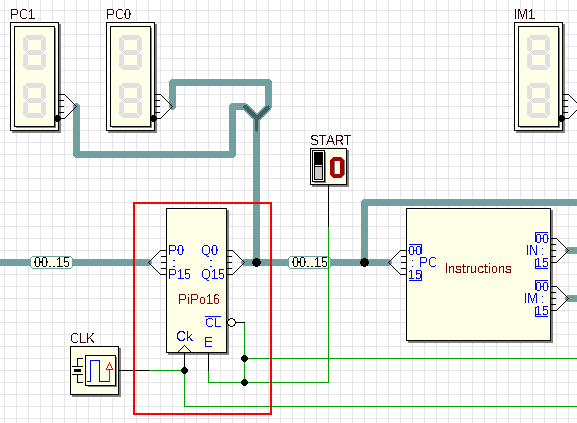
\includegraphics[width=.9\textwidth]{Projeto/images/circuit__instruction_register.png}
    \caption{Zoom no Registrador de Instruções}\label{fig:circuit__instruction_register.png}
\end{figure}

O processador ZeptoProcessador-III segue a mesma ideia de execução do
processador \emph{MIPS} apresentado na figura~\ref{fig:circuit__MIPS.png}
(fonte:~\cite{Digital_Design}). Então é possível ver todas as ligações
relevantes relacionadas ao registrador de instruções.

\begin{figure}[H]
    \centering
    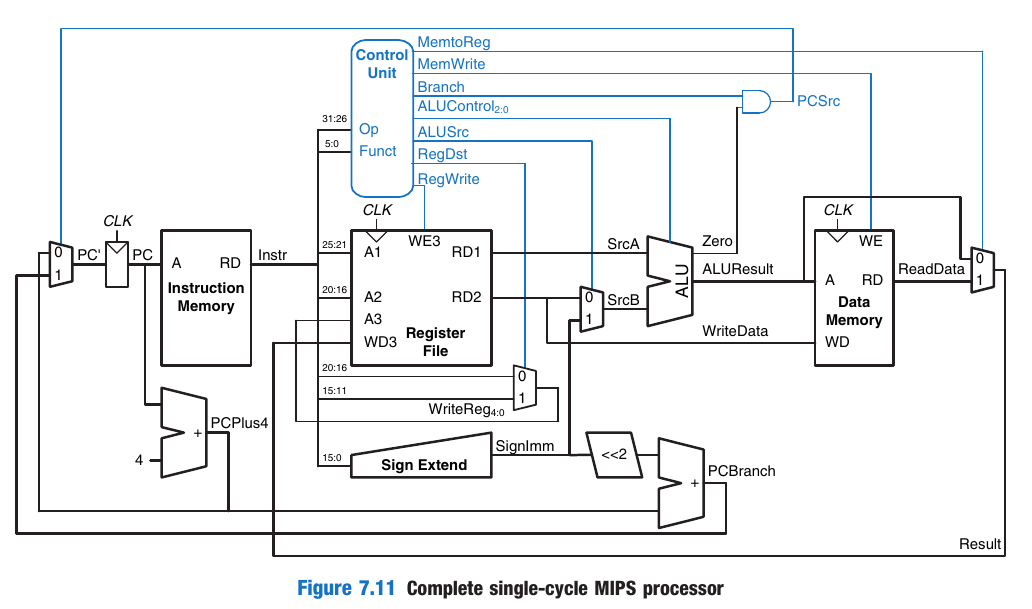
\includegraphics[width=.9\textwidth]{Projeto/images/circuit__MIPS.png}
    \caption{Overview esquemático do processador \emph{MIPS}}\label{fig:circuit__MIPS.png}
\end{figure}

% 2.2
\subsection{Montagem do Circuito da Memória de Instruções}\label{sec:2.2}

Como foi possível observar no circuito do registrador de instruções, o output
daquele circuito se ligava à memória de instruções. Tal componente de um
processador server para armazenar as instruções que um usuário do processador
deseja que este execute. Dessa forma, o processador se torna \emph{programável}.

No ZeptoProcessador-III, a memória de instruções é implementada utilizando-se a
memória ROM. Ela é uma memória somente de leitura, de rápido acesso. Tal tipo de
memória foi muito utilizada por exemplo em cartuchos de \emph{video-games},
\emph{CD}s e afins (para maiores informações sobre essa tecnologia,
consultar~\cite{ROM_memory})

Sua implementação no circuito integrado do processador é dada conforme a
imagem~\ref{fig:circuit__ROM_memory.png}. Pela figura, é possível observar que
existem duas memórias ROM separadas, que recebem como input o endereço produzido
pelo registrador de instruções. O uso de duas memórias ROM separadas se dá
devido ao fato de que, segundo as especificações do ZeptoProcessador-III, a
memória de instruções deve ser capaz de armazenar instruções de $32$
\emph{bits}. Entretanto, como a maior memória ROM disponível no \emph{Deeds} é
de $16$ \emph{bits}, foi utilizado uma memória ROM para armazenar os $16$
\emph{bits} menos significativos, e outra ROM para os outros $16$ \emph{bits}
mais significativos.

\begin{figure}[H]
    \centering
    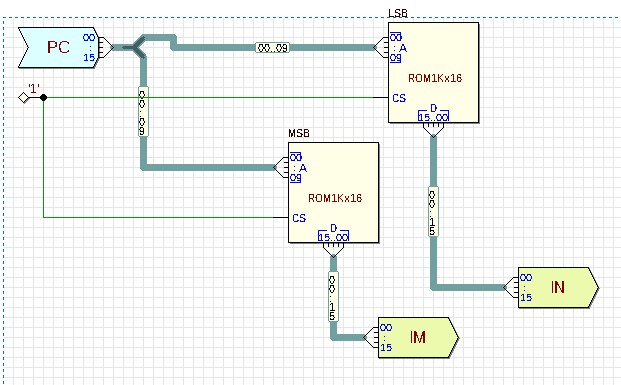
\includegraphics[width=.9\textwidth]{Projeto/images/circuit__ROM_memory.png}
    \caption{Overview da Memória de Instruções}\label{fig:circuit__ROM_memory.png}
\end{figure}

% 2.3
\subsection{Montagem do Circuito do Banco de Registradores}\label{sec:2.3}

O próximo bloco de circuito lógico necessário para um processador funcional é o
\emph{Banco de Registradores}. Tal circuito possibilita o armazenamento de dados
durante a operação do processador, servindo como memória para manipulação de
variáveis e controle de estados.

O ZeptoProcessador-III possui como especificação um banco de registradores
contendo $16$ registradores de $16$ \emph{bits} cada. Além disso,
esquematicamente o banco de registradores funciona da sequinte forma: $3$ canais
de input sinalizam respectivamente o endereço de leitura dos registradores
\emph{Ra}, \emph{Rb} e o endereço de escrita do registrador \emph{Rd}. O banco
de registradores também possui um canal com $16$ \emph{bits} que corresponde aos
dados de escrita, o sinal de \emph{clock}, um sinal para informar se o banco de
registradores deve escrever os dados de escrita no registrador \emph{Rd}, um
sinal de \emph{reset} (que faz com que todos os registradores no banco assumam o
valor $0$), e por fim também possui dois canais de saída de dados \emph{Sa} e
\emph{Sb} que são os dados de leitura dos registradores nos endereços \emph{Ra}
e \emph{Rb}, respectivamente. A figura~\ref{fig:diagram__register_file.png}
(fonte:~\cite{Diagram_Register_file}) mostra esquematicamente como opera um
banco de registradores.

\begin{figure}[H]
    \centering
    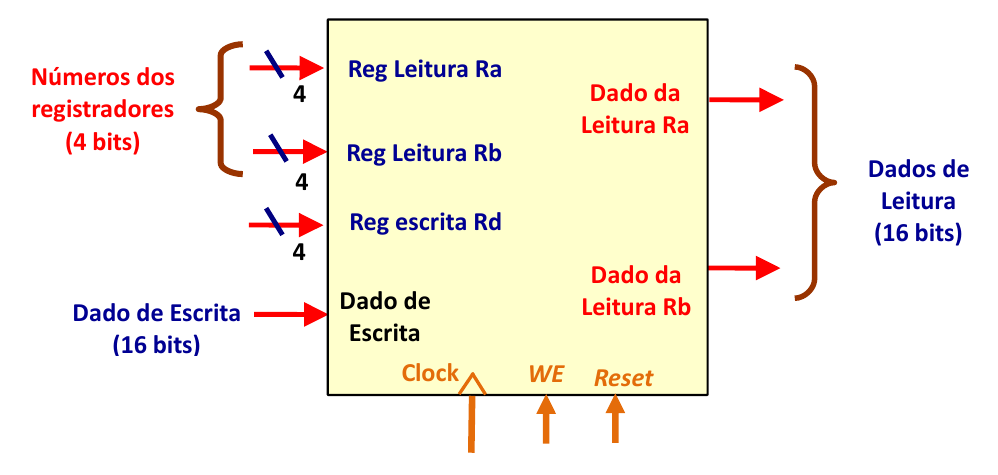
\includegraphics[width=.9\textwidth]{Projeto/images/diagram__register_file.png}
    \caption{Esquema do funcionamento de um Banco de Registradores}\label{fig:diagram__register_file.png}
\end{figure}

E, finalmente, na figura~\ref{fig:circuit__register_file.png} é possível ver
como foi organizado o banco de registradores do ZeptoProcessador-III. Por ser um
circuito muito grande, as figuras~\ref{fig:circuit__register_file_1.png}
e~\ref{fig:circuit__register_file_2.png} mostram, respectivamente, mais
detalhadamente os circuito dos registradores e dos selecionadores de canais
valendo-se de multiplexadores. Novamente, por uma limitação dos blocos
pré-existentes no \emph{Deeds}, a seleção de canais foi feita com dois
multiplexadores de $8$ canais e posteriormente com um multiplexador de $2$
canais devido a ausência de um multiplexador que contenha diretamente $16$
canais.

\begin{figure}[H]
    \centering
    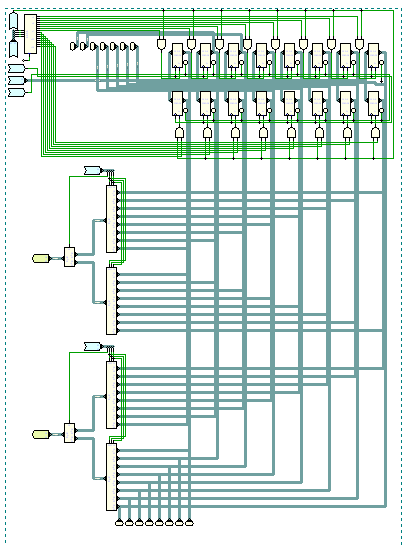
\includegraphics[width=.9\textwidth]{Projeto/images/circuit__register_file.png}
    \caption{Montagem do Banco de Registradores}\label{fig:circuit__register_file.png}
\end{figure}

\begin{figure}[H]
    \centering
    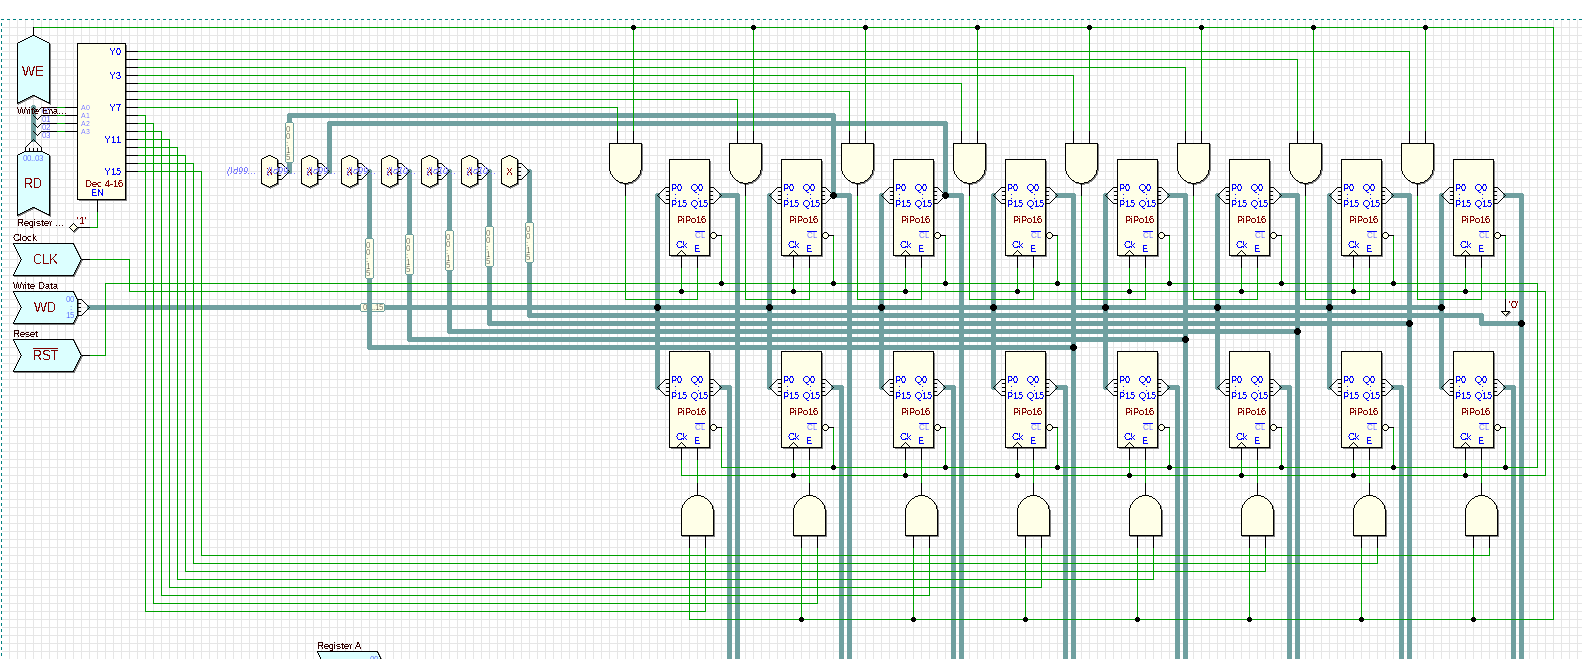
\includegraphics[width=.9\textwidth]{Projeto/images/circuit__register_file_1.png}
    \caption{Zoom nos registradores do banco}\label{fig:circuit__register_file_1.png}
\end{figure}

\begin{figure}[H]
    \centering
    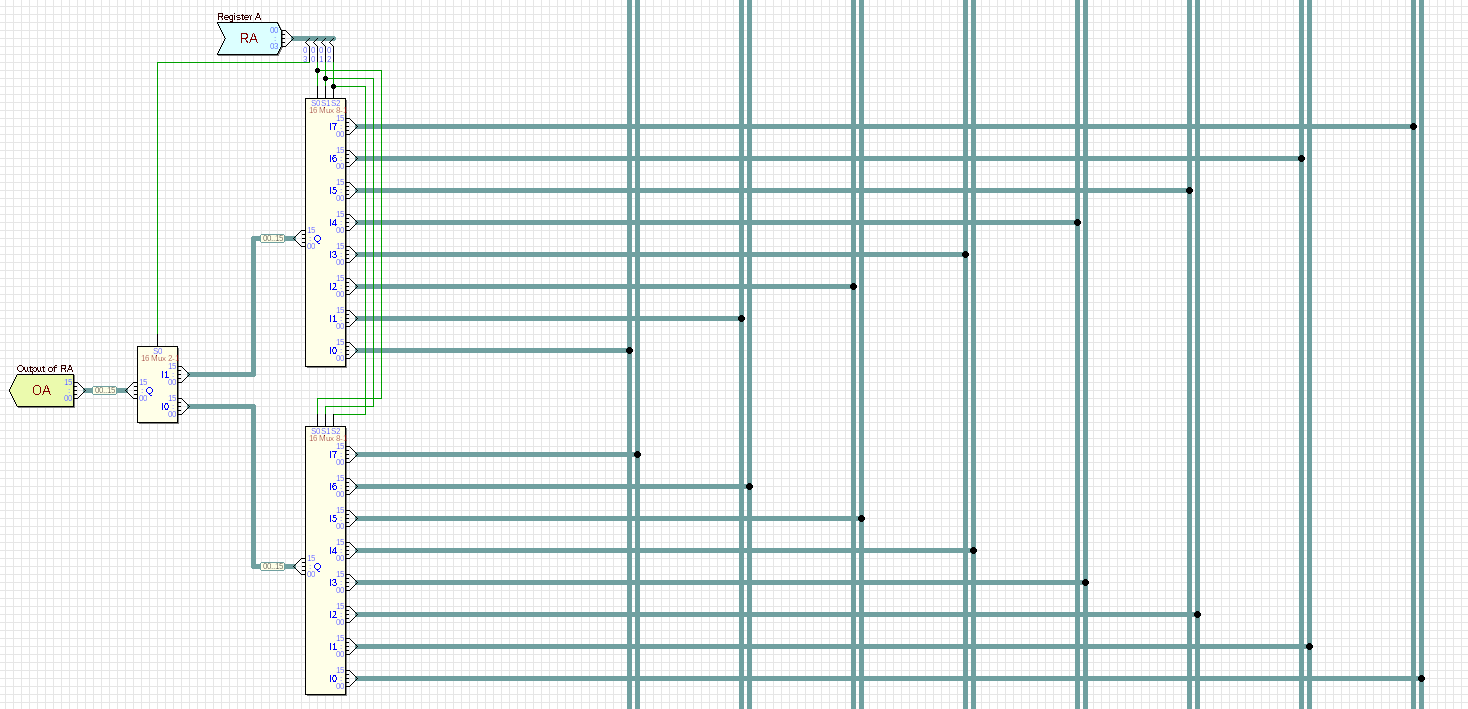
\includegraphics[width=.9\textwidth]{Projeto/images/circuit__register_file_2.png}
    \caption{Zoom no seletor de canais}\label{fig:circuit__register_file_2.png}
\end{figure}


% 2.4
\subsection{\textbf{TODO: Insert Section Title}}\label{sec:2.4}

\textbf{TODO}

\section{Execução de Programas no ZeptoProcessador-III}\label{sec:programs}

\subsection{Multiplicação de Números sem Sinal}\label{sec:programs:multu}

Para o primeiro programa proposto no projeto, faremos um que multiplique dois
números sem sinal, e retorne o valor da multiplicação no registrador \emph{R1}.
Os valores de input para o programa serão carregados nos registradores \emph{R2}
e \emph{R3}, com valores de $8$ e $5$, respectivamente. O resultado esperado da
multiplicação será $8 \cdot 5 = 40$, que, em hexadecimal, corresponde a
$0x0028$.

O código do programa, e seus respectivos comentários, podem ser encontrados na
tabela~\ref{tab:programs:multu}.

\begin{table}[H]
    \centering
    \caption{Código para o programa \textbf{Multu}}
    \begin{tabular}{|l|l|l|l|}\hline
        \textbf{Endereço} & \textbf{Código Hexadecimal} & \textbf{Instrução} & \textbf{Comentário} \\\hline
        0x0000       & 0x0000 0010 & addi R1,R0,R0,0 & R1 = 0 ;; Resultado           \\\hline
        0x0001       & 0x0008 0020 & addi R2,R0,R0,8 & R2 = 8                        \\\hline
        0x0002       & 0x0005 0030 & addi R3,R0,R0,5 & R3 = 5                        \\\hline
        0x0003       & 0x0002 00FB & jal R15,Proc    & R15 = 0x0004; PC=Proc         \\\hline
        0x0004 Fim:  & 0x0000 1105 & beq R1,R1,0     & j Fim ;; mostra R1            \\\hline
        0x0005 Proc: & 0x0000 0040 & addi R4,R0,R0,0 & R4 = 0 ;; instantiate counter \\\hline
        0x0006 Loop: & 0x0000 2110 & addi R1,R1,R2,0 & R1 += R2                      \\\hline
        0x0007       & 0x0001 0440 & addi R4,R4,R0,1 & R4 += 1                       \\\hline
        0x0008       & 0xFFFE 3406 & bne  R4,R3,Loop & if (R4 \!= R3) goto Loop      \\\hline
        0x0009       & 0x0000 0F0C & jalr R0,R15,0   & Retorna resultado em R1       \\\hline
    \end{tabular}\label{tab:programs:multu}
\end{table}

Para a demonstração do programa funcionando, por favor conferir o vídeo no link:
\href{https://youtu.be/NygIUTYyUNY}{https://youtu.be/NygIUTYyUNY}

E, como requisitado, o diagrama de onda do programa pode ser visto na
figura~\ref{fig:program__multu_wave.png}. O processador conseguiu executar o
presente programa na máxima frequência de $4.35MHz$. Qualquer outra frequência
mais rápida que essa resulta em falha no funcionamento, e toda frequência menor
que essa resulta em um resultado sub-ótimo.

\begin{figure}[H]
    \centering
    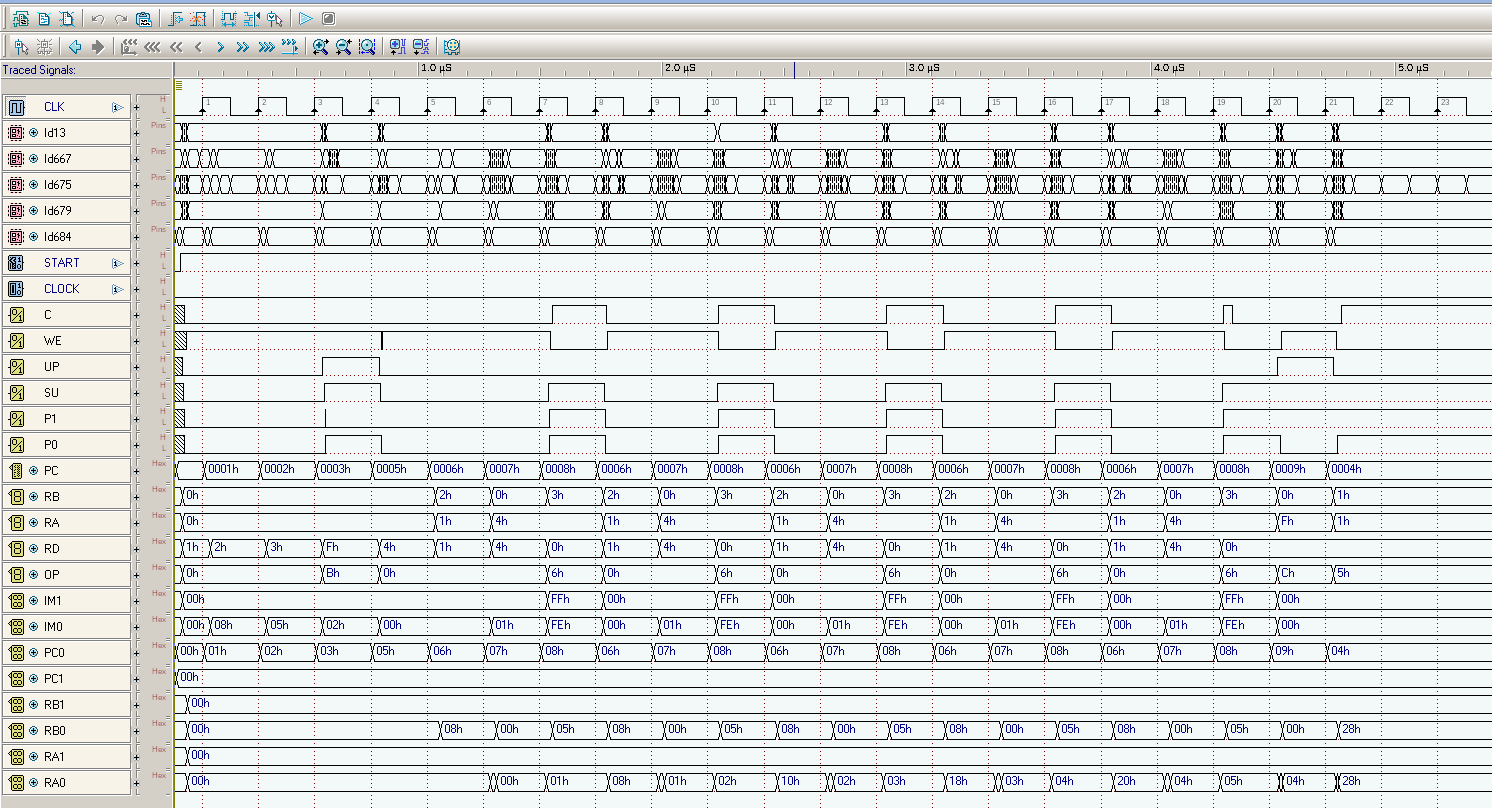
\includegraphics[width=.9\textwidth]{Projeto/images/program__multu_wave.png}
    \caption{Diagrama de onda para o programa Multu}\label{fig:program__multu_wave.png}
\end{figure}

\subsection{Multiplicação de Números com Sinal}\label{sec:programs:mult}

Agora, para o programa de multiplicação de números com sinal, o programa
proposto realiza a multiplicação de dois números com sinal, e retorna o valor da
multiplicação no registrador \emph{R1}. Os valores de input para o programa
serão carregados nos registradores \emph{R2} e \emph{R3}, com valores de $-2$ e
$5$, respectivamente. O resultado esperado da multiplicação será
$-2 \cdot 5 = -10$, que, em hexadecimal, corresponde a $0xFFF6$.

O código do programa, e seus respectivos comentários, podem ser encontrados na
tabela~\ref{tab:programs:mult}.

\begin{table}[H]
    \centering
    \caption{Código para o programa \textbf{Mult}}
    \begin{tabular}{|l|l|l|l|}\hline
        \textbf{Endereço} & \textbf{Código Hexadecimal} & \textbf{Instrução} & \textbf{Comentário}\\\hline
        0x0000        & 0x0000 0010 & addi R1,R0,R0,0      & R1 = 0 ;; Resultado            \\\hline
        0x0001        & 0xFFFE 0020 & addi R2,R0,R0,-2     & R2 = -2                        \\\hline
        0x0002        & 0x0005 0030 & addi R3,R0,R0,5      & R3 = 5                         \\\hline
        0x0003        & 0x0002 00FB & jal  R15,Proc        & R15 = 0x0004; PC=Proc          \\\hline
        0x0004 Fim:   & 0x0000 1105 & beq  R1,R1,0         & j Fim ;; mostra R1             \\\hline
        0x0005 Proc:  & 0x0000 0040 & addi R4,R0,R0,0      & R4 = 0 ;; counter              \\\hline
        0x0006        & 0x8000 0050 & addi R5,R0,R0,0x8000 & R5 (is a mask)                 \\\hline
        0x0007        & 0xFFFF 5262 & andi R6,R2,R5,0xFFFF & R6 == 0x08000 ?                \\\hline
        0x0008        & 0x0004 5606 & bne  R6,R5,R2end     & R6 is a result of a mask       \\\hline
        0x0009        & 0x0001 4040 & addi R4,R0,R4,1      & Increment count of odd numbers \\\hline
        0x000A        & 0xFFFF 0224 & xori R2,R2,R0,0xFFFF & One's compelemnt for R2        \\\hline
        0x000B        & 0x0001 0220 & addi R2,R2,R0,1      & Two's compelemnt for R2        \\\hline
        0x000C R2end: & 0xFFFF 5362 & andi R6,R3,R5,0xFFFF & R6 == 0x08000 ?                \\\hline
        0x000D        & 0x0004 5606 & bne  R6,R5,R3end     & R6 is a result of a mask       \\\hline
        0x000E        & 0x0001 0440 & addi R4,R4,R0,1      & Increment count of odd numbers \\\hline
        0x000F        & 0xFFFF 0334 & xori R3,R3,R0,0xFFFF & One's compelemnt for R3        \\\hline
        0x0010        & 0x0001 0330 & addi R3,R3,R0,1      & Two's compelemnt for R3        \\\hline
        0x0011 R3end: & 0x0000 0070 & addi R7,R0,R0,0      & R7 = 0 ;; loop counter         \\\hline
        0x0012 Loop:  & 0x0000 2110 & addi R1,R1,R2,0      & R1 += R2                       \\\hline
        0x0013        & 0x0001 0770 & addi R7,R7,R0,1      & R7 += 1                        \\\hline
        0x0014        & 0xFFFE 3706 & bne  R7,R3,Loop      & if (R7 \!= R3) goto Loop       \\\hline
        0x0015        & 0x0001 0060 & addi R6,R0,R0,1      & R6 = 1                         \\\hline
        0x0016        & 0x0003 6406 & bne  R4,R6,Ok        & if (R4 \!= R6) goto Ok         \\\hline
        0x0017        & 0xFFFF 0114 & xori R1,R1,R0,0xFFFF & One's complement for R1        \\\hline
        0x0018        & 0x0001 0110 & addi R1,R1,R0,1      & Two's complement for R1        \\\hline
        0x0019 Ok:    & 0x0000 0F0C & jalr R0,R15,0        & Retorna resultado em R1        \\\hline
    \end{tabular}\label{tab:programs:mult}
\end{table}

Para a demonstração do programa funcionando, por favor conferir o vídeo no link:
\href{https://youtu.be/IQj2BHXhxUk}{https://youtu.be/IQj2BHXhxUk}

E, como requisitado, o diagrama de onda do programa pode ser visto na
figura~\ref{fig:program__mult_wave.png}. O processador conseguiu executar o
presente programa na máxima frequência de $4.35MHz$. Qualquer outra frequência
mais rápida que essa resulta em falha no funcionamento, e toda frequência menor
que essa resulta em um resultado sub-ótimo.

\begin{figure}[H]
    \centering
    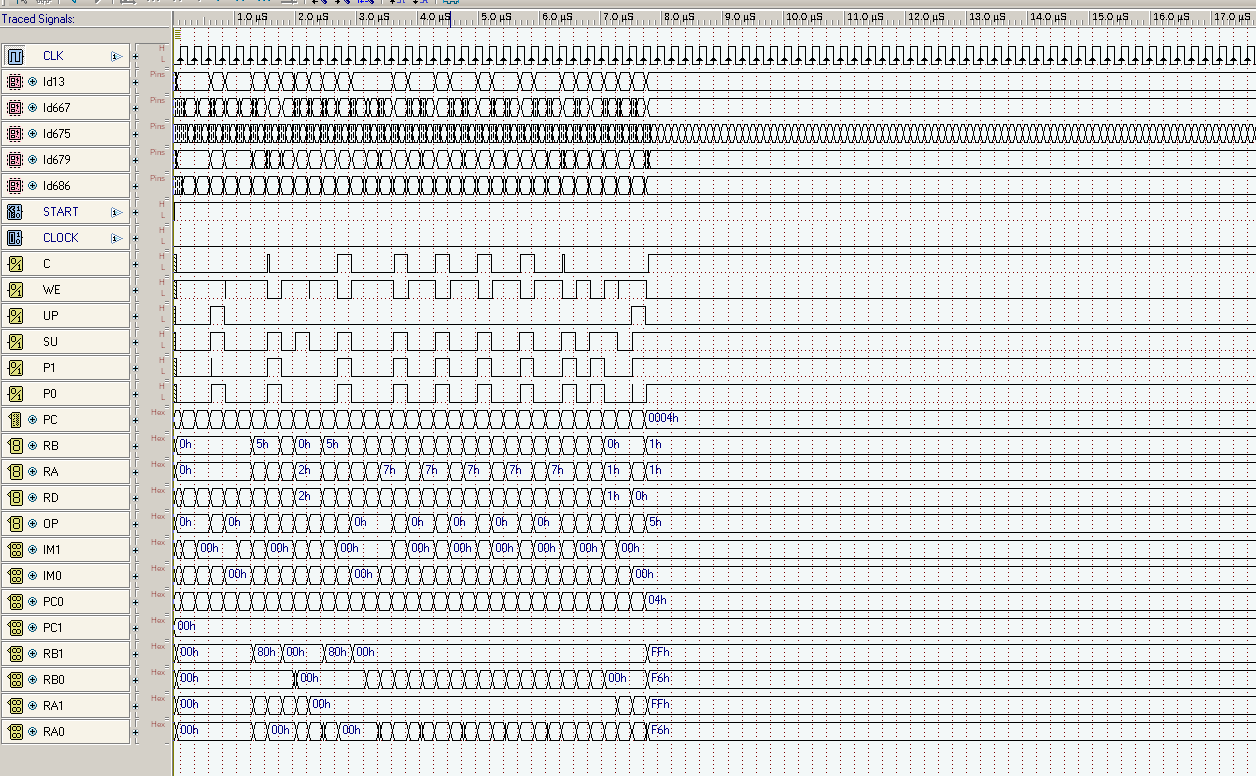
\includegraphics[width=.9\textwidth]{Projeto/images/program__mult_wave.png}
    \caption{Diagrama de onda para o programa Mult}\label{fig:program__mult_wave.png}
\end{figure}

\subsection{Divisão de Números sem Sinal}\label{sec:programs:divu}

Agora, para o programa de divisão de números sem sinal, o programa proposto
realiza a divisão de um número pelo outro, ambos representados sem sinal, e
retorna o valor da divisão no registrador \emph{R1}. Os valores de input para o
programa serão carregados nos registradores \emph{R2} e \emph{R3}, com valores
de $60$ e $12$, respectivamente. O resultado esperado da multiplicação será
$\frac{60}{12} = 5$, que, em hexadecimal, corresponde a $0x0005$.

O código do programa, e seus respectivos comentários, podem ser encontrados na
tabela~\ref{tab:programs:divu}.

Processa a divisão $\frac{60}{12}$. Resultado esperado em R1 = 5.

\begin{table}[H]
    \centering
    \caption{Código para o programa \textbf{Divu}}
    \begin{tabular}{|l|l|l|l|}\hline
        \textbf{Endereço} & \textbf{Código Hexadecimal} & \textbf{Instrução} & \textbf{Comentário} \\\hline
        0x0000       & 0x0000 0010 & addi R1,R0,R0,0  & R1 = 0 ;; Resultado           \\\hline
        0x0001       & 0x003C 0020 & addi R2,R0,R0,60 & R2 = 60                       \\\hline
        0x0002       & 0x000C 0030 & addi R3,R0,R0,12 & R3 = 12                       \\\hline
        0x0003       & 0x0002 00FB & jal R15,Proc     & R15 = 0x0004; PC=Proc         \\\hline
        0x0004 Fim:  & 0x0000 1105 & beq R1,R1,0      & j Fim ;; mostra R1            \\\hline
        0x0005 Proc: & 0x0000 0040 & addi R4,R0,R0,0  & R4 = 0 ;; store the quotient  \\\hline
        0x0006       & 0x0007 230A & bgtu R3,R2,End   & Make sure R2 $>=$ R3           \\\hline
        0x0007 Loop: & 0x0000 3221 & subi R2,R2,R3,0  & R2 -= R3                      \\\hline
        0x0008       & 0x0001 0440 & addi R4,R4,R0,1  & R4 += 1                       \\\hline
        0x0009       & 0xFFFE 320A & bgtu R2,R3,Loop  & if (R2 > R3) goto Loop        \\\hline
        0x000A       & 0x0003 3206 & bne  R2,R3,End   & if (R2 \!= R3) goto End       \\\hline
        0x000B       & 0x0001 0440 & addi R4,R4,R0,1  & R4 += 1                       \\\hline
        0x000C       & 0x0000 0020 & addi R2,R0,R0,0  & R2 = 0                        \\\hline
        0x000D End:  & 0x0000 0410 & addi R1,R4,R0,0  & R1 = R4 ;; get the quotient   \\\hline
        0x000E       & 0x0000 0F0C & jalr R0,R15,0    & Retorna resultado em R1       \\\hline
    \end{tabular}\label{tab:programs:divu}
\end{table}

% Para a demonstração do programa funcionando, por favor conferir o vídeo no link:
% \href{}{}

% E, como requisitado, o diagrama de onda do programa pode ser visto na
% figura~\ref{fig:program__mult_wave.png}. O processador conseguiu executar o
% presente programa na máxima frequência de $4.35MHz$. Qualquer outra frequência
% mais rápida que essa resulta em falha no funcionamento, e toda frequência menor
% que essa resulta em um resultado sub-ótimo.

% \begin{figure}[H]
%     \centering
%     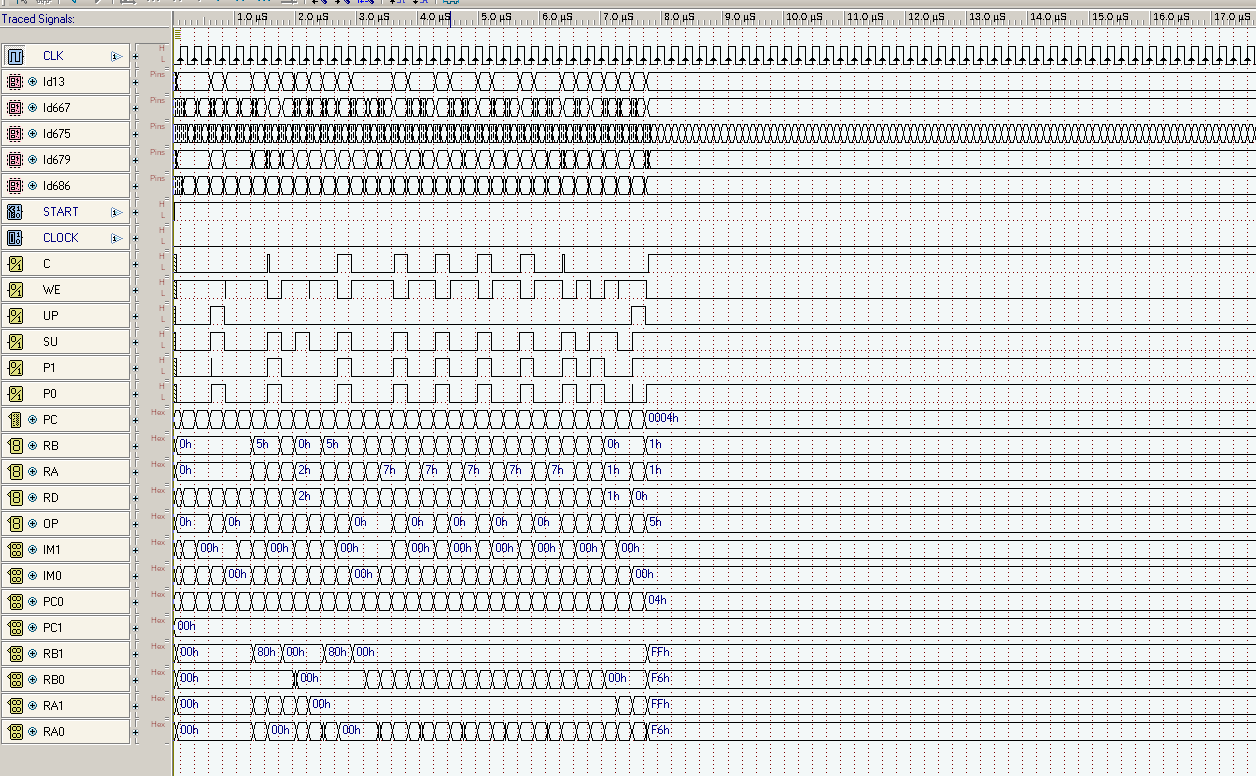
\includegraphics[width=.9\textwidth]{Projeto/images/program__mult_wave.png}
%     \caption{Diagrama de onda para o programa Mult}\label{fig:program__mult_wave.png}
% \end{figure}


\subsection{Divisão de Números com Sinal}\label{sec:programs:div}

Processa a divisão $\frac{60}{12}$. Resultado esperado em R1 = 5.

\begin{table}[H]
    \centering
    \caption{Código para o programa \textbf{Div}}
    \begin{tabular}{|l|l|l|l|}\hline
        \textbf{Endereço} & \textbf{Código Hexadecimal} & \textbf{Instrução} & \textbf{Comentário} \\\hline
        0x0000         & 0x0000 0010 & addi R1,R0,R0,0      & R1 = 0 ;; Resultado                           \\\hline
        0x0001         & 0x0040 0020 & addi R2,R0,R0,64     & R2 = 64                                       \\\hline
        0x0002         & 0x000C 0030 & addi R3,R0,R0,12     & R3 = 12                                       \\\hline
        0x0003         & 0x0002 00FB & jal  R15,Proc        & R15 = 0x0004; PC=Proc                         \\\hline
        0x0004 Fim:    & 0x0000 1105 & beq  R1,R1,0         & j Fim ;; mostra R1                            \\\hline
        0x0005 Proc:   & 0x0000 0040 & addi R4,R0,R0,0      & R4 = 0 ;; store the quotient                  \\\hline
        0x0005         & 0xZZZZ ZZZZ & addi R10,R2,R0,0     & R10 = R2 ;; store for later use               \\\hline
        0x0005         & 0xZZZZ ZZZZ & addi R8,R0,R0,0      & R8 = 0 ;; counter how many negative values    \\\hline
        0xZZZZ         & 0xZZZZ ZZZZ & addi R5,R0,R0,0x8000 & R5 = 0x8000 ;; mask to find negative numbers  \\\hline
        0xZZZZ         & 0xZZZZ ZZZZ & andi R6,R2,R5,0xFFFF & Find if R2 is negative or not                 \\\hline
        0xZZZZ         & 0xZZZZ ZZZZ & bne  R6,R5,R2end     & if (R6 \!= R5) goto R2end                     \\\hline
        0xZZZZ         & 0xZZZZ ZZZZ & addi R8,R8,R0,1      & R8 += 1                                       \\\hline
        0xZZZZ         & 0xZZZZ ZZZZ & xori R2,R2,R0,0xFFFF & One's complement for R2                       \\\hline
        0xZZZZ         & 0xZZZZ ZZZZ & addi R2,R2,R0,1      & Two's complement for R2                       \\\hline
        0xZZZZ R2end:  & 0xZZZZ ZZZZ & andi R7,R3,R5,0xFFFF & Find if R3 is negative or not                 \\\hline
        0xZZZZ         & 0xZZZZ ZZZZ & bne  R7,R5,R3end     & if (R7 \!= R5) goto R3end                     \\\hline
        0xZZZZ         & 0xZZZZ ZZZZ & addi R8,R8,R0,1      & R8 += 1                                       \\\hline
        0xZZZZ         & 0xZZZZ ZZZZ & xori R3,R3,R0,0xFFFF & One's complement for R3                       \\\hline
        0xZZZZ         & 0xZZZZ ZZZZ & addi R3,R3,R0,1      & Two's complement for R3                       \\\hline
        0xZZZZ R3end:  & 0x0007 230A & bgtu R3,R2,End       & Make sure R2 $>=$ R3                          \\\hline
        0xZZZZ Loop:   & 0x0000 3221 & subi R2,R2,R3,0      & R2 -= R3                                      \\\hline
        0xZZZZ         & 0x0001 0440 & addi R4,R4,R0,1      & R4 += 1                                       \\\hline
        0xZZZZ         & 0xFFFE 320A & bgtu R2,R3,Loop      & if (R2 > R3) goto Loop                        \\\hline
        0xZZZZ         & 0x0003 3206 & bne  R2,R3,Prog      & if (R2 \!= R3) goto End                       \\\hline
        0xZZZZ         & 0x0001 0440 & addi R4,R4,R0,1      & R4 += 1                                       \\\hline
        0xZZZZ         & 0x0000 0020 & addi R2,R0,R0,0      & R2 = 0                                        \\\hline
        0xZZZZ Prog:   & 0xZZZZ ZZZZ & addi R9,R0,R0,1      & R9 = 1                                        \\\hline
        0xZZZZ         & 0xZZZZ ZZZZ & bne  R8,R9,Almost    & if (R8 \!= R9) goto Almost                    \\\hline
        0xZZZZ         & 0xZZZZ ZZZZ & addi R4,R4,R0,1      & R4 += 1 ;; add one to the quotient            \\\hline
        0xZZZZ         & 0xZZZZ ZZZZ & subi R2,R3,R101      & R4 += 1                                       \\\hline
        0xZZZZ Almost: & 0xZZZZ ZZZZ & ---------------      & ---------------------------                   \\\hline
        0xZZZZ End:    & 0x0000 0410 & addi R1,R4,R0,0      & R1 = R4 ;; get the quotient                   \\\hline
        0xZZZZ         & 0x0000 0F0C & jalr R0,R15,0        & Retorna resultado em R1                       \\\hline
    \end{tabular}\label{tab:programs:div}
\end{table}

\subsection{Resto da Divisão de Números sem Sinal}\label{sec:programs:remu}

Processa a divisão $\frac{60}{12}$. Resultado esperado em R1 = 5.

\begin{table}[H]
    \centering
    \caption{Código para o programa \textbf{Remu}}
    \begin{tabular}{|l|l|l|l|}\hline
        \textbf{Endereço} & \textbf{Código Hexadecimal} & \textbf{Instrução} & \textbf{Comentário} \\\hline
        0x0000       & 0x0000 0010 & addi R1,R0,R0,0  & R1 = 0 ;; Resultado           \\\hline
        0x0001       & 0x0040 0020 & addi R2,R0,R0,64 & R2 = 64                       \\\hline
        0x0002       & 0x000C 0030 & addi R3,R0,R0,12 & R3 = 12                       \\\hline
        0x0003       & 0x0002 00FB & jal R15,Proc     & R15 = 0x0004; PC=Proc         \\\hline
        0x0004 Fim:  & 0x0000 1105 & beq R1,R1,0      & j Fim ;; mostra R1            \\\hline
        0x0005 Proc: & 0x0000 0040 & addi R4,R0,R0,0  & R4 = 0 ;; store the quotient  \\\hline
        0x0006       & 0x0007 230A & bgtu R3,R2,End   & Make sure R2 $>=$ R3          \\\hline
        0x0007 Loop: & 0x0000 3221 & subi R2,R2,R3,0  & R2 -= R3                      \\\hline
        0x0008       & 0x0001 0440 & addi R4,R4,R0,1  & R4 += 1                       \\\hline
        0x0009       & 0xFFFE 320A & bgtu R2,R3,Loop  & if (R2 > R3) goto Loop        \\\hline
        0x000A       & 0x0003 3206 & bne  R2,R3,End   & if (R2 \!= R3) goto End       \\\hline
        0x000B       & 0x0001 0440 & addi R4,R4,R0,1  & R4 += 1                       \\\hline
        0x000C       & 0x0000 0020 & addi R2,R0,R0,0  & R2 = 0                        \\\hline
        0x000D End:  & 0x0000 0210 & addi R1,R2,R0,0  & R1 = R2 ;; get the remainder  \\\hline
        0x000E       & 0x0000 0F0C & jalr R0,R15,0    & Retorna resultado em R1       \\\hline
    \end{tabular}\label{tab:programs:remu}
\end{table}

\section{Análise dos Resultados}\label{sec:resultados}

Passaremos a analisar individualmente cada um dos tópicos anteriores, levantando
observações pertinentes para cada um deles.

\subsection{Análise do tópico~\ref{sec:2.1}}\label{sec:analise2.1}

\textbf{TODO}

\subsection{Análise do tópico~\ref{sec:2.2}}\label{sec:analise2.2}

\textbf{TODO}

\subsection{Análise do tópico~\ref{sec:2.3}}\label{sec:analise2.3}

\textbf{TODO}

\subsection{Análise do tópico~\ref{sec:2.4}}\label{sec:analise2.4}

\textbf{TODO}

\section{Conclusão}\label{sec:Conclusao}

\textbf{TODO}

\bibliographystyle{sbc}
\bibliography{relatorio}  %Aqui é a definição do arquivo .bib a ser usado pelas referências

\end{document}
